\documentclass{article}
\usepackage[utf8]{inputenc}
\usepackage{amsmath}
\usepackage{amsfonts}
\usepackage{esint}
\usepackage{geometry}
\usepackage{color}
\usepackage{fancyhdr}
\usepackage{ctable}
\usepackage{fancybox}
\usepackage{tabularx}
\usepackage{array}
\usepackage{booktabs}
\usepackage[french]{babel}
\usepackage{dsfont}
\usepackage{setspace}
\usepackage[french]{minitoc}
\usepackage{multicol}
\usepackage{multirow}
\usepackage[hidelinks]{hyperref}
\usepackage{graphicx}
\usepackage[T1]{fontenc}
\usepackage{xcolor}
\usepackage{listings}

\geometry{top=2.5cm, bottom=2.5cm, left=3cm, right=3cm}

\addtocounter{tocdepth}{3}
\setcounter{secnumdepth}{3}


\definecolor{codegreen}{rgb}{0,0.6,0}
\definecolor{codegray}{rgb}{0.5,0.5,0.5}
\definecolor{codepurple}{rgb}{0.58,0,0.82}
\definecolor{backcolour}{rgb}{0.95,0.95,0.92}

\lstdefinestyle{mystyle}{
  backgroundcolor=\color{white}, commentstyle=\color{codegreen},
  keywordstyle=\color{magenta},
  numberstyle=\tiny\color{codegray},
  stringstyle=\color{codepurple},
  basicstyle=\ttfamily\footnotesize,
  breakatwhitespace=false,         
  breaklines=true,                 
  captionpos=b,                    
  keepspaces=true,                 
  numbers=left,                    
  numbersep=5pt,                  
  showspaces=false,                
  showstringspaces=false,
  showtabs=false,                  
  tabsize=2
}

\lstset{style=mystyle}

\begin{document}

%%%%%%%%%%%%%%%%%%%%%%%%%%%%%%%%%%%%%%%%%%%%%%%%%%%%%%
%%%%%%%%%%%%%%%%%%%% PRÉSENTATION %%%%%%%%%%%%%%%%%%%%
%%%%%%%%%%%%%%%%%%%%%%%%%%%%%%%%%%%%%%%%%%%%%%%%%%%%%%

\begin{titlepage}

    \unitlength 1cm
    \begin{center}
    
    \vspace*{1cm}

    
\includegraphics[scale=0.6]{figures/logo_ico.png}
    
    \vspace{2cm}
    
               {\Large Diplôme de Qualification en Physique Radiologique et Médicale\\}
               
    \vspace{2cm}           
    
    
    \rule{16cm}{0.7pt}
    
    \vspace{12pt}
               
               {\LARGE \bf Faisceaux de photons de haute énergie : cas des petits faisceaux\\}
               
    \vspace{12pt}
    \rule{16cm}{0.7pt}

    \vspace{2cm}

                {\large Fiche n°3b}
    
    \vspace{1.5cm}

               {\Large\bf {Alexandre \textsc{Rintaud}}}
    
    \vspace{1.5cm}
    
    \end{center}
    
    Encadrants :
    
    \small {
    \begin{tabular}{llr}\\
    \textbf{Stéphanie \textsc{Josset}}   &  &  \\
      Physicienne médicale, \textsc{Centre René Gauducheau ICO, Saint Herblain} &    &  \\
    
    \end{tabular}
    }

    \vspace{1.5cm}


    \begin{center}
    \textsc{Semestre 3 2024}
    \end{center}
    
\end{titlepage}
\let\cleardoublepage\clearpage


%%%%%%%%%%%%%%%%%%%%%%%%%%%%%%%%%%%%%%%%%%%%%%%%%%%%%%
%%%%%%%%%%%%%%%%%%%%%%% STYLE %%%%%%%%%%%%%%%%%%%%%%%%
%%%%%%%%%%%%%%%%%%%%%%%%%%%%%%%%%%%%%%%%%%%%%%%%%%%%%%

\onehalfspacing

%Style  du corps
\pagestyle{fancy}
	\renewcommand\headrulewidth{0.5pt}
	\renewcommand\footrulewidth{0.5pt}
	\fancyfoot[L]{\textsc{A. Rintaud}}
	\fancyfoot[C]{\textsc{ICO Nantes}}
	\fancyfoot[R]{\thepage}

\tableofcontents
\clearpage
\section{Introduction}

La radiothérapie externe utilise, de manière prépondérante, les faisceux de photons de haute énergie afin de traiter des cellules cancéreuses tout en épargnant le plus possible les tissus sains. Dans cette optique, la connaissance précise des caractéristiques dosimétriques ainsi que les incertitudes associées de l'accélérateur utilisé sont nécessaires. 

Ce rapport traitera des faisceaux de photons utilisés en radiothérapie. Premièrement, le matériel et les méthodes utilsiés lors des mesures des doses absolues basées sur les protocoles internationaux fournis par l'Agence Internationale de l'Énergie Atomique (AIEA) seront explicités, puis les résultats seront présentés. 

\section{Matériels et méthodes}

Cette partie est consacrée à la mesure de la dose absorbée dans les conditions de référence, telles que décrites dans le protocole TRS-398 de l'AIEA \cite{international2001iaea}. De plus, nous développerons également la méthodologie du protocole TRS-277 \cite{internationaliaea}.

\subsection{Facteurs correctifs}

L'utilisation d'une chambre d'ionnisation à cavité d'air étanche pour la mesure de la dose absolue engendre une fluctuation de la réponse du système de mesure en fonction de plusieurs paramètres. Il faut donc appliquer une correction de la mesure grâce à l'équation suivante :

\begin{equation}
  M_{Q}^{'} = M_Q \times k_{T,P} \times k_{pol} \times k_{rec} \times k_H
  \label{eq_corr_charge}
\end{equation}

Avec $M_Q$ la charge mesurée sur l'électromètre, $k_{T,P}$ le facteur correctif de la pression et de la température, $k_{pol}$ le facteur correctif de la polarisation de la chambre, $k_{rec}$ le facteur correctif de la recombinaison ionique et $k_H$ le facteur correctif des conditions hygrométriques.

\subsubsection{Pression et température}

Le facteur $k_{T,P}$ permet de corriger de la pression et de la température et se calcule de la manière suivante :

\begin{equation}
  k_{T,P} = \dfrac{P_0T}{T_0P}
  \label{eq_k_TP}
\end{equation}

Avec $P_0$ et $T_0$ la pression et la température de référence, respectivement égales à 1013,25 hPa et 273,15 K, $P$ et $T$ sont la pression et la température de la salle lors de la mesure.

\subsubsection{Polarisation}

Ce facteur correctif, noté $k_{pol}$, permet de corriger de l'effet de la polarité appliquée à la chambre lors de la mesure :

\begin{equation}
  k_{pol} = \dfrac{|M_+| + |M_-|}{2M}
  \label{eq_pol}
\end{equation}

Avec $M_+$ et $M_-$ les charges mesurées pour les tensions $V_+$ et $V_-$ respectivement et $M$ est la réponse pour la tension utilisée en clinique.

\subsubsection{Recombinaisons ioniques}

Le facteur de recombinaison permet de corriger la réponse de la chambre d'ionisation sur le nombre de charges collectées. La mesure est sous estimée car des paires d'ions sont recombinées et ne rentrent pas en compte dans la mesure.

\begin{equation}
  k_{rec} = a_0 + a_1 \left(\dfrac{M_1}{M_2}\right) + a_2 \left(\dfrac{M_1}{M_2}\right) ^2
  \label{eq_rec}
\end{equation}

Avec $M_1$ et $M_2$ les réponses aux tensions $V_1$ et $V_2$ respectivement, et $a_0$, $a_1$ et $a_2$ sont les facteurs tabulés en fonction du rapport $\frac{V_1}{V_2}$ fournis par le protocole TRS-398 \cite{international2001iaea}.

\subsubsection{Humidité}

Ce facteur est égale à 1 lorsque l'humidité de la salle est comprise entre 20\% et 80\%, sinon il faut lui attribuer la valeur de 0,997.

\subsection{Indice de qualité}

L'indice de qualité est calculé de la manière suivante :

\begin{equation}
  IQ = TPR^{20}_{10} = \dfrac{D_{20 \, cm}}{D_{10 \, cm}}
  \label{eq_iq}
\end{equation}

Avec $D_{10 \, cm}$ la dose mesurée à 10 cm de profondeur et $D_{20 \, cm}$ la dose mesurée à 20 cm de profondeur.

La distance source détecteur (DSD) doit être constante entre les deux mesures, comme le montre la figure \ref*{fig_tpr} :

\begin{figure}[h]
  \centering
  \includegraphics[scale=0.27]{figures/iq_schema.png}
  \caption{Conditions géométriques pour la mesure du l'indice de qualité}
  \label{fig_tpr}
\end{figure}

\subsection{Protocole TRS-277}

La mesure de la dose absolue est définie, selon le protocole TRS 277 de l'AIEA \cite{internationaliaea}, à partir de l'équation suivante :

\begin{equation}
  D_{eau, Q} = M_Q N_{K_{air, \, Q_0}} k_{att} k_{m} (1-g) \left(\dfrac{S}{\rho}\right)^{eau}_{air} p_u p_{cel}
  \label{eq_dose_277}
\end{equation}

Avec :

\begin{itemize}
  \item[$\bullet$] $M_Q$ la charge mesurée par la chambre
  \item[$\bullet$] $N_{K_{air, \, Q_0}}$ le coefficient d'étalonnage de la chambre en kerma dans l'air pour un faisceau de qualité $Q_0$ (généralement $Q_0  =\: ^{60}$Co)
  \item[$\bullet$] $k_{att}$ le facteur corrigeant de l'atténuation et de la diffusion dues à la paroi de la chambre
  \item[$\bullet$] $k_m$ le facteur correctif de la non-équivalence à l'air de la paroi et du capuchon de mise en équilibre électronique
  \item[$\bullet$] $g$ la fraction d'énergie perdue par radiation (rayonnement de freinage des particules secondaires)
  \item[$\bullet$] $\left(\dfrac{S}{\rho}\right) ^{eau}_{air}$ le rapport entre le pouvoir d'arrêt massique de l'eau et celui de l'air pour les particules primaires
  \item[$\bullet$] $p_u$ facteur de correction de perturbation
  \item[$\bullet$] $p_{cel}$ facteur de correction de l'électrode centrale
\end{itemize}

Le facteur $p_u$ peut se décomposer en un produit de facteurs :

\begin{equation}
  p_{u,\, Q} = p_{wall,\, Q} \times p_{cav,\, Q} \times p_{dist,\, Q}
  \label{eq_pu}
\end{equation}

Avec :
\begin{itemize}
  \item[$\bullet$] $p_{wall,\, Q}$ facteur correctif de la non équivalence à l'eau de la paroi
  \item[$\bullet$] $p_{cav,\, Q}$ facteur corrigeant de la non homogénéité de la cavité
  \item[$\bullet$] $p_{dist,\, Q}$ facteur permettant de corriger le déplacement d'un volume d'eau provoqué par la présence de la chambre
\end{itemize}

\subsection{Protocole TRS-398}

Le protocole TRS 398 de l'AIEA \cite{international2001iaea} permet de calculer la dose absorbée dans l'eau dans les conditions de référence tout en simplifiant le formalisme de calcul du TRS 277. La dose absorbée est donnée par la formule suivante :

\begin{equation}
  D_{eau,\, Q} = M_{Q}^{'} \times N_{D_{eau},\, Q_0} \times k_{Q,\, Q_0}
  \label{eq_dose_398}
\end{equation}

Avec :
\begin{itemize}
  \item[$\bullet$] $M_{Q}^{'}$ la mesure de la charge corrigée des facteurs $k_{T,P}$ $k_{pol}$ $k_{rec}$ et $k_H$
  \item[$\bullet$] $N_{D_{eau},\, Q_0}$ le coefficient d'étalonnage de la chambre en dose dans l'eau à l'aide d'un faisceau de qualité $Q_0$ 
  \item[$\bullet$] $k_{Q,\, Q_0}$ le coefficient de correction de la qualité faisceau
\end{itemize}

\begin{equation}
  k_{Q,\, Q_0} = \dfrac{N_{D_{eau},\, Q}}{N_{D_{eau},\, Q_0}} = \dfrac{D_{air,\, Q} \left[\left(\dfrac{S}{\rho}\right) ^{eau}_{air}\right]_Q p_Q M_{Q_0}}{D_{air,\, Q_0 } \left[\left(\dfrac{S}{\rho}\right) ^{eau}_{air}\right]_{Q_0} p_{Q_0} M_Q}
\end{equation}

L'estimation du facteur $k_{Q,\, Q_0}$ est donné en fonction du type de chambre et de la qualité du faisceau en Annexe \ref*{fig_table_kQQ0}.

\newpage
\subsection{Erreurs de positionnement}

Nous avons également réalisé des mesures pour mesurer l'impact d'un mauvais positionnement de la chambre. Pour cela, nous avons appliqué un déplacement de 1 mm dans la direction latérale de part et d'autre du point de référence, puis de 1 mm en profondeur au dessus et en dessous de ce même point. Dix mesures on été faites pour chaque énergie et chaque position pour ensuite calculer la charge moyenne. La dose est ensuite calculée selon le protocole TRS-398 de l'AIEA \cite{international2001iaea} puis un écart relatif est calculé entre la dose de référence et celle calculée avec le déplacement de 1 mm.

\subsection{Incertitudes}

\subsubsection{Incertitudes de type A}

Les incertitudes de type A sont liées à l'analyse d'une série d'observations qui se répètent en se fondant sur la distribution statistique des résultats. L'incertitude-type $u(x)$ associé à une série de $n$ résultats $x_i$ est donnée par :

\begin{equation}
  u(x) = \sqrt{\dfrac{\sum\limits_{i=1}^n (x_i - \overline{x})^2}{n-1}}
\end{equation}

Si le résultat recherché est la moyenne arithmétique de $n$ observations indépendantes répétées, l'incertitude-type sur la moyenne est donné par l'estimateur $s(\overline{x})$, qui est l'écart-type expérimental de la moyenne :

\begin{equation}
  u(\overline{x}) = \dfrac{u(x)}{\sqrt{n}} = \sqrt{\dfrac{\sum\limits_{i=1}^n (x_i - \overline{x})^2}{n(n-1)}}
\end{equation}

\subsubsection{Incertitudes de type B}

Les incertitudes de type B sont basées sur des connaissances scientifiques du phénomène observé qui peuvent être :

\begin{itemize}
  \item[$\bullet$] des données antérieures mesurées
  \item[$\bullet$] des spécifications du constructeur
  \item[$\bullet$] des données fournies lors d'un étalonnage ou d'autres certifications
  \item[$\bullet$] des incertitudes issues de données de références extraites de tables
  \item[$\bullet$] des propriétés du matériel utilisé
\end{itemize}

Pour donner quelques exemples, si la grandeur $X$ observée peut prendre des valeurs restreintes dans un intervalle [$x - a$, $x + a$] et que la distribution est uniforme, alors l'u-incertitude-type associée est :

\begin{equation}
  u(x) = \dfrac{a}{\sqrt{3}}
\end{equation}

Si la grandeur $X$ observée est dans un intervalle bien défini mais qui n'est pas au centre de celui-ci, l'incertitude-type associée est donnée par :

\begin{equation}
  u(x) = \dfrac{a}{12}
\end{equation}

Cette deuxième situation est le cas d'une lecture de la température ou de la pression sur un thermomètre ou un baromètre respectivement et $a$ correspond à la graduation de l'outil de mesure.

\subsubsection{Propagation des incertitudes}

Dans notre cas, la dose absorbée se calcule en pultipliant plusieurs facteurs entre eux. Dans cette situation, l'incertitude-type associée à la dose absolue est régie par l'éuation suivante :

\begin{equation}
  \dfrac{u(y)}{y} = \sqrt{\sum\limits_i^n \left( \dfrac{u(x_i)}{x_i} \right) ^2}
\end{equation}

\subsubsection{Incertitude élargie}

Pour répondre à certaines exigences, l'incertitude-type peut être multipliée par un coefficent d'élargissement $k$. Cette pratique sert à fournir un intervalle à l'interieur duquel se situe une large pproportion de la distribution des valeurs qui peuvent être associées au mesurande. Dans ce travail, le facteur d'élargissement $k$ sera pris égal à 2 pour s'assurer que la vraie valeur se trouve dans l'intervalle défini par les incertitudes-types calculées avec une probabilité de 95 \%.


\subsection{Contrôle du débit de référence (TOP)}

Quotidiennement, un contôle qualité est réalisé sur les accélérateurs, communément appelé TOP. Ce contrôle permet de vérifier la dérive du débit dans le temps sur un faisceau fixe dans les conditions de référence (champ 10x10 cm$^2$, mesure faite à 10 cm de profondeur et DSD = 100 cm comme le montre la figure \ref*{fig_top}). 

\begin{figure}[h]
  \centering
  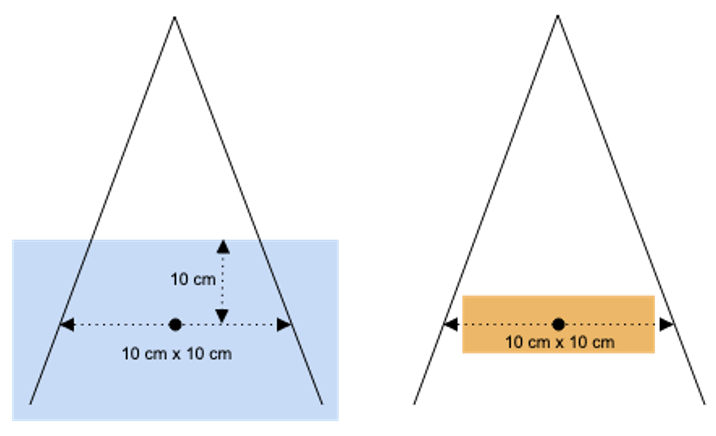
\includegraphics[scale=0.8]{figures/conditions_ref_top.png}
  \caption{Conditions de mesures de la dose absorbée dans la cuve à eau (à gauche) et dans le bloc TOP (à droite)}
  \label{fig_top}
\end{figure}

La dose dans ces conditions est d'abord mesurée dans la cuve à eau, puis un facteur de passage entre l'eau et le bloc TOP est appliqué pour mesurer la dose dans le bloc lors des contrôles quotidiens. Ce facteur $f$ est défini comme suit :

\begin{equation}
  f = \dfrac{D_0}{M_0}
  \label{eq_facteur_top}
\end{equation}

Avec $D_0$ la dose mesurée dans les conditions de référence (Gy) et $M_0$ la mesure de la charge (nC) dans la boîte à TOP.

La dose du jour lors du contrôle qualité se calcule de la façon suivante :

\begin{equation}
  D_j = M_j \times \dfrac{D_0}{M_0} \times k_{TP} = M_j \times f \times k_{TP}
  \label{eq_top_jour}
\end{equation}

Avec $M_j$ la mesure de la charge du jour $j$ dans la boîte à TOP, $f = \frac{D_0}{M_0}$ le facteur de passage de la cuve à eau à la boîte à TOP et $k_{TP}$ le facteur de correction de la pression et de la température donné par la formule \ref*{eq_k_TP}.

\clearpage
\section{Résultats}
\subsection{Détermination des facteurs correctifs}

Le calcul des différents facteurs de correction de la mesure ont été calculés par les formules \ref*{eq_k_TP}, \ref*{eq_pol} et \ref*{eq_rec} (pour la pression et la température, la polarité et la recombinaison ionique) dont les résultats sont indiqués dans les tableaux \ref*{table_ktp} et \ref*{table_kpol}. Concernant la recombinaison ionique, les coefficients $a_0$, $a_1$ et $a_2$ sont indiqués dans le tableau \ref*{table_facteurs_krec}. Ces coefficients sont tirés du protocole TRP-398 de l'AIEA \cite{international2001iaea} représentés sur la figure \ref*{fig_krec}. L'ensemble des mesures de dose absolue ont été réalisées sur le Clinac 2.

\begin{table}[h]
  \centering
  \begin{tabular}{ccc}
    \toprule
    \textbf{Température (K)} & \textbf{Pression (hPa)} & $\mathbf{k_{TP}}$ \\
    \toprule
    21 & 1015 & 1,0017 \\
    \bottomrule
  \end{tabular}
  \caption{Calcul du $k_{TP}$}
  \label{table_ktp}
\end{table}


\begin{table}[h]
  \centering
  \begin{tabular}{c|cccc|cccc|}
  \cline{2-9}
                                                     & \multicolumn{4}{c|}{\textbf{X6}} & \multicolumn{4}{c|}{\textbf{X23}} \\ \hline
  \multicolumn{1}{|c|}{\textbf{Tension (V)}} & \textbf{400} & \textbf{100} & \textbf{-400} & \textbf{-100} & \textbf{400} & \textbf{100} & \textbf{-400} & \textbf{-100} \\ \hline
  \multicolumn{1}{|c|}{\textbf{Charge 1 (nC)}}       & 29,69  & 29,50  & 29,80  & 29,61 & 36,64  & 36,15  & 36,78  & 36,28  \\
  \multicolumn{1}{|c|}{\textbf{Charge 2 (nC)}}       & 29,70   & 29,52  & 29,82  & 29,59 & 36,62  & 36,10  & 36,75  & 36,25  \\
  \multicolumn{1}{|c|}{\textbf{Charge 3 (nC)}}       & 29,73  & 29,55  & 29,80  & 29,61 & 36,61  & 36,08  & 36,73  & 36,21  \\
  \multicolumn{1}{|c|}{\textbf{Charge moyenne (nC)}} & 29,71  & 29,52  & 29,81  & 29,60 & 36,62  & 36,11  & 36,75  & 36,25  \\ \hline
  \multicolumn{1}{|c|}{$\mathbf{k_{rec}}$}                & \multicolumn{4}{c|}{1,0020}      & \multicolumn{4}{c|}{1,0046}       \\
  \multicolumn{1}{|c|}{$\mathbf{k_{pol} \, 400 \, V}$}          & \multicolumn{4}{c|}{1,0019}      & \multicolumn{4}{c|}{1,0019}       \\
  \multicolumn{1}{|c|}{$\mathbf{k_{pol} \, 100 \, V}$}          & \multicolumn{4}{c|}{1,0014}      & \multicolumn{4}{c|}{1,0019}       \\ 
  \multicolumn{1}{|c|}{\textbf{Écart relatif} $\mathbf{k_{pol}}$ \textbf{\%}} & \multicolumn{4}{c|}{0,05} & \multicolumn{4}{c|}{0} \\
  \hline
  \end{tabular}
  \caption{Série de mesures pour le calcul du $k_{rec}$ et du $k_{pol}$ pour des faisceaux de photons de 6 MV et 23 MV (Clinac 2)}
  \label{table_kpol}
\end{table}



\begin{table}[h]
  \centering
  \begin{tabular}{cccc}
    \toprule
    $\mathbf{\frac{V_1}{V_2}}$ & $\mathbf{a_0}$ & $\mathbf{a_1}$ & $\mathbf{a_2}$\\
    \toprule
    4 & 1,022 & -0,363 & 0,341\\
    \bottomrule    
  \end{tabular}
  \caption{Facteurs tabulés correspondant au rapport $\frac{V_1}{V_2}$}
  \label{table_facteurs_krec}
\end{table}

\begin{figure}[h!]
  \centering
  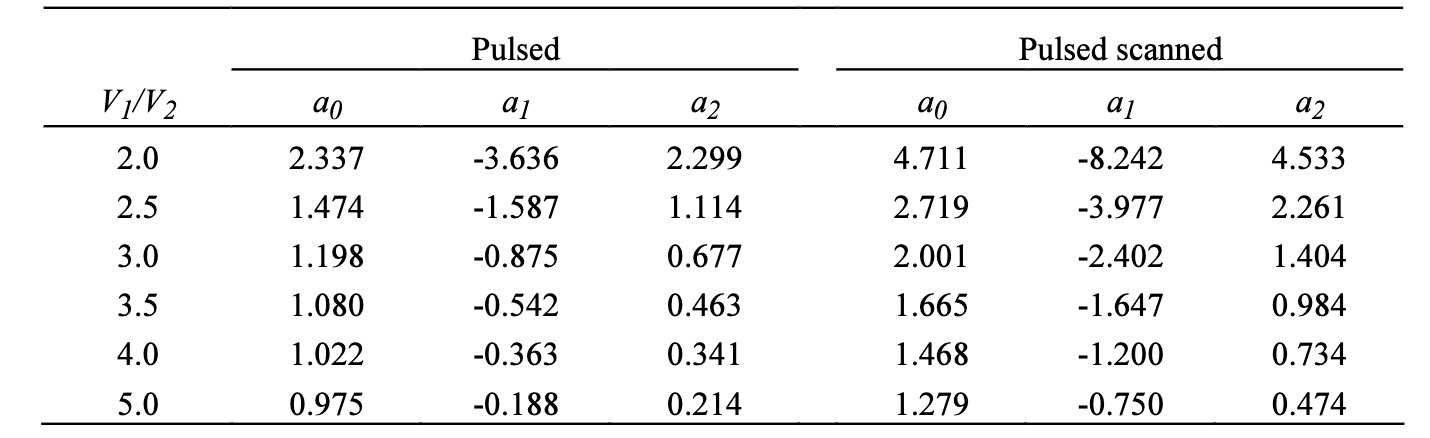
\includegraphics[scale=0.5]{figures/coeff_krec.png}
  \caption{Coefficients d'extrapolation pour le calcul du $k_{rec}$ par la technique des "deux tensions", en fonction du rapport $V_1/V_2$}
  \label{fig_krec}
\end{figure}

\newpage
\subsection{Mesure de l'indice de qualité}

L'indice de qualité est calculé pour les deux énergies disponibles sur le Clinac 2 (6 MV et 23 MV). Il a été calculé à l'aide de l'équation \ref*{eq_iq}. Nous avons réalisé 10 mesures de charge pour chaque énergie et chaque profondeur. Les valeurs moyennes ont été utilisées pour le calcul de l'indice de qualité, comme le montre le tableau \ref*{table_resultats_tpr}.

\begin{table}[h]
  \centering
  \begin{tabular}{c|cc|cc|}
  \cline{2-5}
  \textbf{} & \multicolumn{2}{c|}{\textbf{X6}} & \multicolumn{2}{c|}{\textbf{X23}} \\ \cline{2-5} 
  \textbf{} & \textbf{10 cm} & \textbf{20 cm} & \textbf{10 cm} & \textbf{20 cm} \\ \hline
  \multicolumn{1}{|c|}{\textbf{Charge moyenne   (nC)}} & 29,66 & 19,67 & 36,59 & 28,54 \\
  \hline
  \multicolumn{1}{|c|}{$\mathbf{TPR^{20}_{10}}$ \textbf{mesuré}} & \multicolumn{2}{c|}{0,663} & \multicolumn{2}{c|}{0,780} \\
  \multicolumn{1}{|c|}{$\mathbf{TPR^{20}_{10}}$ \textbf{recette}} & \multicolumn{2}{c|}{0,664} & \multicolumn{2}{c|}{0,781} \\
  \multicolumn{1}{|c|}{\textbf{ER (\%)}} & \multicolumn{2}{c|}{0,125} & \multicolumn{2}{c|}{0,133} \\ \hline
  \end{tabular}
  \caption{Résultats de la mesure du $TPR^{20}_{10}$ pour des faisceaux de photons de 6 MV et de 23 MV (Clinac 2)}
  \label{table_resultats_tpr}
\end{table}

L'indice de qualité est très légèrement sous estimé quelle que soit l'énergie du faisceau avec des écarts relatif de 0,125 \% et de 0,133 \% respectivement pour les faisceaux X6 et X23.

\subsection{Mesure de la dose absolue de référence}

La messure de la dose absolue se base, dans nos manipulations, sur le protocole TRS-398 \cite{international2001iaea}. Les mesures de dose ont été réalisées sur les deux énergies disponibles sur le Clinac 2 (6 MV et 23 MV) et pour deux chambres d'ionnisation étalonnées récemment : PTW  Farmer de 0,6 cm$^3$ et PTW Pinpoint de 0,03 cm$^3$ comme indiqué sans le tableau \ref*{table_dose_abs_resultats}.

\begin{table}[h!]
  \centering
  \begin{tabular}{c|cc|cc|}
  \cline{2-5}
                                             & \multicolumn{2}{c|}{\textbf{X6}}    & \multicolumn{2}{c|}{\textbf{X23}}   \\ \cline{2-5} 
                                             & \textbf{Farmer} & \textbf{Pinpoint} & \textbf{Farmer} & \textbf{Pinpoint} \\ \hline
  \multicolumn{1}{|c|}{\textbf{Charge moyenne (nC)}} & 29,66           & 0,675             & 36,59           & 0,8311            \\
  \multicolumn{1}{|c|}{\textbf{$\mathbf{N_{D_{eau},\, Q_0}}$ (Gy/nC)}} & 5,356$\times 10^{-2}$ & 2,344 & 5,356$\times 10^{-2}$ & 2,344                     \\
  \multicolumn{1}{|c|}{\textbf{$\mathbf{k_{Q,\, Q_0}}$}}       & \multicolumn{2}{c|}{0,9966}   & \multicolumn{2}{c|}{0,9767}                       \\
  \multicolumn{1}{|c|}{\textbf{Dose mesurée (Gy)}}   & 1,595           & 1,596             & 1,933            & 1,930             \\
  \multicolumn{1}{|c|}{\textbf{Dose recette (Gy)}}             & \multicolumn{2}{c|}{1,589}    & \multicolumn{2}{c|}{1,907}                        \\
  \multicolumn{1}{|c|}{\textbf{Écart relatif (\%)}}            & 0,35                  & 0,44  & 1,35                  & \multicolumn{1}{l|}{1,21} \\ \hline
  \end{tabular}
  \caption{Résultats de la dose absolue dans les conditions de référence avec les chambres Farmer et Pinpoint pour des faisceaux de 6 MV et 23 MV (Clinac 2)}
  \label{table_dose_abs_resultats}
\end{table}

Les résultats que nous obtenons sont proches de ceux obtenus lors de la recette, quelle que soit l'énergie du faisceau ainsi que la chambre d'ionisation utilisée lors de la mesure bien que les volumes sensibles des deux chambres utilisées soient très différents.

\newpage
\subsection{Incertitudes}

Le tableau \ref*{table_incertitudes_abs} synthétise les incertitudes associées au calcul de la dose absolue dans les conditions de références.

\begin{table}[h]
  \centering
  \begin{tabular}{c|cccc|cccc|}
  \cline{2-9}
   &
    \multicolumn{4}{c|}{\textbf{Farmer}} &
    \multicolumn{4}{c|}{\textbf{Pinpoint}} \\ \cline{2-9} 
   &
    \multicolumn{2}{c|}{\textbf{X6}} &
    \multicolumn{2}{c|}{\textbf{X23}} &
    \multicolumn{2}{c|}{\textbf{X6}} &
    \multicolumn{2}{c|}{\textbf{X23}} \\ \hline
  \multicolumn{1}{|c|}{\textbf{Type d'incertitude}} &
    \textbf{A} &
    \multicolumn{1}{c|}{\textbf{B}} &
    \textbf{A} &
    \textbf{B} &
    \textbf{A} &
    \multicolumn{1}{c|}{\textbf{B}} &
    \textbf{A} &
    \textbf{B} \\
  \multicolumn{1}{|c|}{\textbf{Charge collectée (\%)}} &
    0,091 &
    \multicolumn{1}{c|}{} &
    0,041 &
     &
    0,125 &
    \multicolumn{1}{c|}{} &
    0,035 &
     \\
  \multicolumn{1}{|c|}{$\mathbf{k_{rec}}$ \textbf{(\%)}} &
     &
    \multicolumn{1}{c|}{0,110} &
     &
    0,108 &
     &
    \multicolumn{1}{c|}{0,058} &
     &
    0,101 \\
  \multicolumn{1}{|c|}{$\mathbf{k_{pol}}$ \textbf{(\%)}} &
     &
    \multicolumn{1}{c|}{0,080} &
     &
    0,080 &
     &
    \multicolumn{1}{c|}{0,032} &
     &
    0,093 \\
  \multicolumn{1}{|c|}{$\mathbf{k_{TP}}$ \textbf{(\%)}} &
     &
    \multicolumn{1}{c|}{0,275} &
     &
    0,275 &
     &
    \multicolumn{1}{c|}{0,275} &
     &
    0,275 \\
  \multicolumn{1}{|c|}{$\mathbf{N_{D_{eau}}}$ \textbf{(\%)}} &
     &
    \multicolumn{1}{c|}{0,55} &
     &
    0,55 &
     &
    \multicolumn{1}{c|}{0,55} &
     &
    0,55 \\
  \multicolumn{1}{|c|}{$\mathbf{k_{Q,\, Q_0}}$ \textbf{(\%)}} &
     &
    \multicolumn{1}{c|}{1} &
     &
    1 &
     &
    \multicolumn{1}{c|}{1} &
     &
    1 \\
  \multicolumn{1}{|c|}{\textbf{Incertiture totale (\%)}} &
    \multicolumn{2}{c|}{1,185} &
    \multicolumn{2}{c|}{1,182} &
    \multicolumn{2}{c|}{1,182} &
    \multicolumn{2}{c|}{1,182} \\ \hline
  \multicolumn{1}{|c|}{\textbf{Incertitude totale élargie (\%)}} &
    \multicolumn{2}{c|}{2,371} &
    \multicolumn{2}{c|}{2,365} &
    \multicolumn{2}{c|}{2,365} &
    \multicolumn{2}{c|}{2,365} \\ \hline
  \end{tabular}
  \caption{Incertitudes associées au calcul de la dose absolue pour des faisceaux de 6 MV et de 23 MV (Clinac 2)}
  \label{table_incertitudes_abs}
\end{table}

Concernant les incertitudes associées aux mesures, le tableau \ref*{table_incertitudes_abs} nous donne une valeur élargie d'un facteur $k=2$ de 2,371 \% maximum.

\subsection{Erreurs de positionnement}

Les tableaux \ref*{table_erreur_lat} et \ref*{table_erreur_profondeur} rendent compte de l'impact sur la dose d'un mauvais positionnement de 1 mm que ce soit dans les directons parallèle ou perpendiculaire au faisceau. Les tableaux \ref*{table_mesure_dep_lat} et \ref*{table_mesure_dep_prof}, en annexe, fournissent l'ensemble des valeurs mesurées ainsi que leur moyenne. Nous pouvons voir qu'un tel déplacement reste presque négligeable dans les deux directions même si l'effet d'un déplacement en profondeur est un peu plus important puisque la loi de l'inverse carré de la distance rentre en jeu ici.  

\begin{table}[h]
  \centering
  \begin{tabular}{c|cc|cc|}
  \cline{2-5}
  \textbf{} & \multicolumn{2}{c|}{\textbf{X6}} & \multicolumn{2}{c|}{\textbf{X23}} \\ \cline{2-5} 
  \textbf{} & \textbf{1 mm} & \textbf{-1 mm} & \textbf{1 mm} & \textbf{-1 mm} \\ \hline
  \multicolumn{1}{|c|}{\textbf{Charge moyenne   (nC)}} & 29,785 & 29,783 & 36,69 & 36,652 \\
  \multicolumn{1}{|c|}{\textbf{Ecart type (nC)}} & 0,015 & 0,019 & 0,018 & 0,019 \\ \hline
  \multicolumn{1}{|c|}{\textbf{Dose (Gy)}} & 1,600 & 1,600 & 1,937 & 1,935 \\
  \multicolumn{1}{|c|}{\textbf{Incertitude absolue (Gy)}} & 0,019 & 0,019 & 0,023 & 0,023 \\
  \multicolumn{1}{|c|}{\textbf{Incertitude relative (\%)}} & 1,182 & 1,182 & 1,178 & 1,182 \\
  \multicolumn{1}{|c|}{\textbf{Incertitude k=2 (\%)}} & 2,364 & 2,365 & 2,356 & 2,363 \\
  \multicolumn{1}{|c|}{\textbf{Ecart (mGy)}} & 5,798 & 5,691 & 4,366 & 2,359 \\
  \multicolumn{1}{|c|}{\textbf{Écart relatif (\%)}} & 0,364 & 0,357 & 0,226 & 0,122 \\ \hline
  \end{tabular}
  \caption{Erreurs de positionnement engendrées par un déplacement latéral de la chambre}
  \label{table_erreur_lat}
\end{table}

\begin{table}[h]
  \centering
  \begin{tabular}{c|cc|cc|}
  \cline{2-5}
  \textbf{} & \multicolumn{2}{c|}{\textbf{X6}} & \multicolumn{2}{c|}{\textbf{X23}} \\ \cline{2-5} 
  \textbf{} & \textbf{101 mm} & \textbf{109 mm} & \textbf{101 mm} & \textbf{109 mm} \\ \hline
  \multicolumn{1}{|c|}{\textbf{Charge moyenne   (nC)}} & 29,553 & 29,868 & 36,470 & 36,756 \\
  \multicolumn{1}{|c|}{\textbf{Ecart type (nC)}} & 0,018 & 0,019 & 0,012 & 0,005 \\
  \multicolumn{1}{|c|}{\textbf{Dose (Gy)}} & 1,588 & 1,605 & 1,925 & 1,941 \\
  \multicolumn{1}{|c|}{\textbf{Incertitude absolue (Gy)}} & 0,019 & 0,019 & 0,023 & 0,023 \\
  \multicolumn{1}{|c|}{\textbf{Incertitude relative (\%)}} & 1,182 & 1,182 & 1,179 & 1,181 \\
  \multicolumn{1}{|c|}{\textbf{Incertitude k=2 (\%)}} & 2,364 & 2,365 & 2,357 & 2,361 \\
  \multicolumn{1}{|c|}{\textbf{Écart (mGy)}} & 6,667 & 10,258 & 7,249 & 7,850 \\
  \multicolumn{1}{|c|}{\textbf{Écart relatif (\%)}} & 0,418 & 0,643 & 0,375 & 0,406 \\ \hline
  \end{tabular}
  \caption{Erreurs de positionnement engendrées par un déplacement en profondeur de la chambre}
  \label{table_erreur_profondeur}
\end{table}

\newpage
\subsection{Contrôle du débit de référence (TOP)}

Le tableau \ref*{table_coeff_passage} résume les résultats obtenus pour le calcul de la dose dans la boîte à TOP. La dose dans l'eau mesurée dans la cuve à eau a été utilsée pour calculer le coefficient de passage pour chacune des énergies du Clinac 2. 

\begin{table}[h]
  \centering
  \begin{tabular}{>{\centering\arraybackslash}m{2cm}>{\centering\arraybackslash}m{2.5cm}>{\centering\arraybackslash}m{2.5cm}>{\centering\arraybackslash}m{2cm}>{\centering\arraybackslash}m{2cm}>{\centering\arraybackslash}m{2cm}}
    \toprule
    \textbf{Date} & \textbf{Énergie (MV)} & \textbf{Dose eau (Gy)} & \textbf{Charge TOP (nC)} & \textbf{Coefficient (Gy/nC)} & \textbf{Écart (\%)}\\
    \toprule
    14/09/2023 & 6 & 1,601 & 25,88 & 6,19$\times$ 10$^{-2}$ & \\
    24/02/2023 & 6 & 1,589 & / & 6,065$\times$ 10$^{-2}$ & 2,06 \\
    \hline
    14/09/2023 & 23 & 1,974 & 32,06 & 6,16$\times$ 10$^{-2}$ & \\
    24/02/2023 & 23 & 1,907 & / & 5,908$\times$ 10$^{-2}$ & 4,27 \\
    \bottomrule
  \end{tabular}
  \caption{Résultats des coefficients de passage pour les deux faisceaux de photons disponibles sur le Clinac 2}
  \label{table_coeff_passage}
\end{table}

Nous observons un écart jusqu'à 4,27 \% entre le coefficient calculé lors des mesures et celui du mois de février. Cette différence s'explique par le fait que pour le coefficient du mois de février, la dose dans l'eau choisie pour le calcul était celle de la recette (1,589 Gy) alors que la dose sélectionnée pour celui de septembre est la dose dans l'eau mesurée lors de nos mesures (1,601 Gy). Si nous calculons l'écart entre les deux coefficient en prenant toujours la dose de la recette comme référence, nous obtenons les résultats donnés dans le tableau \ref*{table_vrai_ecart_coeff}.

\begin{table}[h]
  \centering
  \begin{tabular}{cccc}
    \toprule
    \textbf{Date} & \textbf{Énergie (MV)} & \textbf{Coefficient (Gy/nC)} & \textbf{Écart (\%)} \\
    \toprule
    14/09/2023 & 6 & 6,14$\times$ 10$^{-2}$ & \\
    24/09/2023 & 6 & 6.07$\times$ 10$^{-2}$ & 1,15 \\
    \hline
    14/09/2023 & 23 & 5,95$\times$ 10$^{-2}$ & \\
    24/02/2023 & 23 & 5,91$\times$ 10$^{-2}$ & 0,68 \\
    \bottomrule
  \end{tabular}
  \caption{Écart entre le coefficient de février et celui de septembre à partir de la dose de la recette}
  \label{table_vrai_ecart_coeff}
\end{table}

L'écart entre les deux coefficients fournis par le tableau \ref*{table_vrai_ecart_coeff} est en dessous des 2\% pour les faisceaux de 6 MV et de 23 MV. La dose délivrée par le faisceau est donc stable dans le temps quelle que soit l'énergie de celui-ci.

\clearpage
\section{Annexe}

\begin{figure}[h]
  \centering
  \includegraphics[scale=0.4]{figures/tableau_corr_faisceau.png}
  \caption{Valeurs calculées du $k_{Q,\, Q_0}$ pour les faisceaux de photons de haute énergie}
  \label{fig_table_kQQ0}
\end{figure}

\begin{table}[h]
  \centering
  \begin{tabular}{c|cc|cc|}
  \cline{2-5}
                                                                & \multicolumn{2}{c|}{\textbf{X6}} & \multicolumn{2}{c|}{\textbf{X23}} \\ \cline{2-5} 
  \textbf{}                                                     & \textbf{10 cm}  & \textbf{20 cm} & \textbf{10 cm}  & \textbf{20 cm}  \\ \hline
  \multicolumn{1}{|c|}{\multirow{10}{*}{\textbf{Mesures (nC)}}} & 29,7            & 19,7           & 36,58           & 28,6            \\
  \multicolumn{1}{|c|}{}                                        & 29,66           & 19,67          & 36,57           & 28,54           \\
  \multicolumn{1}{|c|}{}                                        & 29,66           & 19,66          & 36,58           & 28,51           \\
  \multicolumn{1}{|c|}{}                                        & 29,69           & 19,7           & 36,57           & 28,52           \\
  \multicolumn{1}{|c|}{}                                        & 29,66           & 19,66          & 36,58           & 28,52           \\
  \multicolumn{1}{|c|}{}                                        & 29,63           & 19,65          & 36,62           & 28,53           \\
  \multicolumn{1}{|c|}{}                                        & 29,63           & 19,66          & 36,58           & 28,53           \\
  \multicolumn{1}{|c|}{}                                        & 29,63           & 19,68          & 36,6            & 28,53           \\
  \multicolumn{1}{|c|}{}                                        & 29,64           & 19,65          & 36,58           & 28,54           \\
  \multicolumn{1}{|c|}{}                                        & 29,69           & 19,66          & 36,59           & 28,53           \\ \hline
  \multicolumn{1}{|c|}{\textbf{Charge moyenne   (nC)}}          & 29,66           & 19,67          & 36,59           & 28,54           \\ \hline
  \end{tabular}
  \caption{Ensemble des valeurs mesurées pour le calcul de l'indice de qualité}
  \label{table_mesures_IQ}
\end{table}

\begin{table}[h]
  \centering
  \begin{tabular}{c|cc|cc|}
  \cline{2-5}
  \textbf{}                                                     & \multicolumn{2}{c|}{\textbf{X6}} & \multicolumn{2}{c|}{\textbf{X23}} \\ \cline{2-5} 
  \textbf{}                                                     & \textbf{1 mm}     & \textbf{-1 mm}     & \textbf{1 mm}      & \textbf{-1 mm}     \\ \hline
  \multicolumn{1}{|c|}{\multirow{10}{*}{\textbf{Mesures (nC)}}} & 29,76          & 29,75           & 36,66           & 36,66           \\
  \multicolumn{1}{|c|}{} & 29,76 & 29,79 & 36,66 & 36,66 \\
  \multicolumn{1}{|c|}{} & 29,80 & 29,75 & 36,68 & 36,61 \\
  \multicolumn{1}{|c|}{} & 29,78 & 29,80 & 36,69 & 36,63 \\
  \multicolumn{1}{|c|}{} & 29,80 & 29,78 & 36,69 & 36,65 \\
  \multicolumn{1}{|c|}{} & 29,79 & 29,80 & 36,70 & 36,65 \\
  \multicolumn{1}{|c|}{} & 29,79 & 29,80 & 36,70 & 36,66 \\
  \multicolumn{1}{|c|}{} & 29,78 & 29,79 & 36,71 & 36,66 \\
  \multicolumn{1}{|c|}{} & 29,79 & 29,79 & 36,71 & 36,67 \\
  \multicolumn{1}{|c|}{} & 29,80 & 29,78 & 36,70 & 36,67 \\ \hline
  \multicolumn{1}{|c|}{\textbf{Charge moyenne   (nC)}}          & 29,785         & 29,783          & 36,69           & 36,652          \\ \hline
  \end{tabular}
  \caption{Ensemble des valeurs mesurées pour le calcul des incertitudes de déplacement latéral}
  \label{table_mesure_dep_lat}
\end{table}

\begin{table}[h]
  \centering
  \begin{tabular}{c|cc|cc|}
  \cline{2-5}
  \textbf{} & \multicolumn{2}{c|}{\textbf{X6}} & \multicolumn{2}{c|}{\textbf{X23}} \\ \cline{2-5} 
  \textbf{} & \textbf{101 mm} & \textbf{109 mm} & \textbf{101 mm} & \textbf{109 mm} \\ \hline
  \multicolumn{1}{|c|}{\multirow{10}{*}{\textbf{Mesures (nC)}}} & 29,53 & 29,88 & 36,46 & 36,76 \\
  \multicolumn{1}{|c|}{} & 29,55 & 29,83 & 36,45 & 36,75 \\
  \multicolumn{1}{|c|}{} & 29,56 & 29,88 & 36,46 & 36,76 \\
  \multicolumn{1}{|c|}{} & 29,57 & 29,89 & 36,46 & 36,75 \\
  \multicolumn{1}{|c|}{} & 29,54 & 29,87 & 36,47 & 36,75 \\
  \multicolumn{1}{|c|}{} & 29,56 & 29,86 & 36,48 & 36,76 \\
  \multicolumn{1}{|c|}{} & 29,56 & 29,88 & 36,47 & 36,76 \\
  \multicolumn{1}{|c|}{} & 29,52 & 29,84 & 36,48 & 36,75 \\
  \multicolumn{1}{|c|}{} & 29,57 & 29,87 & 36,48 & 36,76 \\
  \multicolumn{1}{|c|}{} & 29,57 & 29,88 & 36,49 & 36,76 \\ \hline
  \multicolumn{1}{|c|}{\textbf{Charge moyenne   (nC)}} & 29,553 & 29,868 & 36,470 & 36,756 \\ \hline
  \end{tabular}
  \caption{Ensemble des valeurs mesurées pour le calcul des incertitudes de déplacement en profondeur}
  \label{table_mesure_dep_prof}
  \end{table}

\clearpage
\bibliography{biblio}
\addcontentsline{toc}{section}{Références}
\bibliographystyle{plain}
\nocite{*}

\end{document}